%
% File acl2015.tex

\documentclass[11pt]{article}
\usepackage{acl2015}
\usepackage{times}
\usepackage{url}
\usepackage{dsfont}
\usepackage{latexsym}
\usepackage{graphicx}


\title{Document Classification by Inversion of \\Distributed Language Representations}

\author{Matt Taddy \\
  University of Chicago Booth School of Business \\
  {\tt taddy@chicagobooth.edu} \\}

\date{}

\begin{document}
\maketitle
\begin{abstract}
There have been many recent advances in the structure and measurement of {\it distributed} language models: those that map from words to a vector-space that is rich in information about word choice and composition.  This vector-space is the distributed language representation.    

Given the success of such approaches,  researchers have proposed
models and algorithms to adapt them for use in document classification; e.g., for predicting sentiment.  The goal of this note is to point out that any distributed  representation can be turned into a classifier through inversion via Bayes rule.  
The approach is simple and modular, in that it will work with any language representation whose training can be formulated as optimizing a probability model. In our application to 2 million sentences from Yelp reviews, we also find that it performs as well as or better than  complex purpose-built algorithms. \end{abstract}

\section{Introduction}

Distributed, or vector-space, language representations $\mathcal{V}$ consist
of a location for every vocabulary {\it word} in $\mathds{R}^K$, where $K$ is
the dimension of the latent representation space.  These locations are learned
to optimize (or approximately optimize) an objective function defined on the
original text, such as a likelihood for word occurrences.

A popular example is the Word2Vec machinery of
Mikolov et al.~\shortcite{mikolov_distributed_2013}.  This trains the distributed
representation to be useful as an input layer for prediction of words from
their neighbors in a Skip-gram likelihood.  That is, to maximize
\begin{equation}\label{eq:skipgram}
\sum_{k\neq t,~j=t-b}^{t+b} \log\mathrm{p}_{\mathcal{V}}(w_{sj}\mid w_{st})
\end{equation}
summed across all words $w_{st}$ in all sentences $\mathbf{w}_s$, where $b$ is
the skip-gram window (possibly truncated by the end or beginning of the
sentence) and the function $\mathrm{p}_{\mathcal{V}}(w_{sj}| w_{st})$ is a neural network
classifier that takes vector-space representations for $w_{st}$ and $w_{sj}$
as input (see Section \ref{sec:w2v}).

Distributed language representations have been studied since the early work on
neural networks \cite{rumelhart_learning_1986} and have long been applied in
natural language processing \cite{morin_hierarchical_2005}.  The models are
generating much recent interest due to the large performance gains from the
newer systems, including Wor2Vec and the Glove model of Pennington et
al.~\shortcite{pennington_glove:_2014}, observed in tasks such as word
prediction, word analogy identification, and named entity recognition.

Given the success of these new models, researchers have begun searching for
ways to adapt the representations for use in document classification tasks
such as sentiment prediction or author identification.  One  naive approach is be
to use aggregated word vectors across a document (e.g., a document's average
word-vector location) as input to a standard classifier (e.g.,
logistic regression).  However, a document is actually  an {\it ordered} path
of  locations through $\mathds{R}$, and simple averaging destroys much of the available
information.  

More sophisticated aggregation is proposed in Socher et al.
\shortcite{socher_parsing_2011,socher_recursive_2013}, where recursive neural
networks are used to combine the word vectors through the estimated parse tree
for each sentence.  Alternatively,  Le and Mikolov's Doc2Vec
\shortcite{le_distributed_2014} adds document labels to the conditioning set
in (\ref{eq:skipgram}) and has them influence the skip-gram likelihood through
a latent input vector location in $\mathcal{V}$. In each case, the end product
is a distributed representation for every sentence (or document for Doc2Vec)
that can be used as input to a generic classifier.

\subsection{Bayesian Inversion}

These approaches all add considerable model and estimation complexity to the
original underlying distributed representation. They require careful
engineering and are not just add-ons to existing systems.   We are proposing a
simple alternative that turns fitted distributed language representations into
document classifiers without any additional modeling or estimation.  

Write the probability model that the representation $\mathcal{V}$ has been
trained to optimize (likelihood maximize) as $\mathrm{p}_{ \mathcal{V}}(d )$,
where document $d = \{\mathbf{w}_1, ... \mathbf{w}_S\}$ is a set of sentences 
-- ordered vectors of word identities.  
For example, in Word2Vec the skip-gram likelihood in
(\ref{eq:skipgram}) yields
\begin{equation}\label{eq:fulllhd}
\log\mathrm{p}_{ \mathcal{V}}(d) = \sum_s \sum_{t} \sum_{k\neq t,~j=t-b}^{t+b} 
\log\mathrm{p}_{ \mathcal{V}_y}(w_{sj}\mid w_{st} ).
\end{equation}
Even when such a likelihood is not explicit it will be implied by the objective function that is optimized during training.

Now suppose that your training documents are grouped by class label, $y \in
\{1 \dots C\}$.  We can train {\it separate} distributed language representations
for each set of documents as partitioned by $y$; for example, fit Word2Vec independently on each sub-corpus $D_c = \{ d_i : y_i =c \}$ and obtain the labeled distributed representation map $\mathcal{V}_c$.  A new  document $d$ has probability
$\mathrm{p}_{ \mathcal{V}_c}(d)$ if we treat it as a member of class $c$, and Bayes rule implies
\begin{equation}\label{eq:bayesrule}
\mathrm{p}( y | d) = \frac{\mathrm{p}_{ \mathcal{V}_y}(d)\pi_y }
{\sum_c \mathrm{p}_{ \mathcal{V}_c}(d)\pi_c }
\end{equation}
where $\pi_c$ is our prior probability on class label $c$.

Thus distributed language representations trained separately for each class label 
yield directly a document classification rule via (\ref{eq:bayesrule}).  This
approach has a number of attractive qualities.

\vskip .2cm
\noindent \textbf{Modularity:} The inversion strategy works for any model of language that can (or its training can) be interpreted as a probabilistic model.  This makes for easy implementation in any system that has already been engineered to fit such language representations.  In business, this will lead to faster deployment and lower costs.  In acadmenia, this can help foster transparency and replicability.

\vskip .2cm
\noindent \textbf{Scalability:}  for massive corpora it becomes necessary split the data into pieces for use in distributed computing.
Our model of classification via inversion provides a clear top-level
partitioning of the data.  Thus an efficient system could be designed to fit separate by-class language representations, which will provide for document classification as in this article as well as class-specific answers for NLP tasks such as word prediction or analogy.  When one wishes to treat a document as unlabeled, NLP tasks can be answered through an ensemble aggregation of the class-specific answers.

\vskip .2cm
\noindent \textbf{Performance:} although it was not our primary goal, we do find that inversion of Word2Vec outperforms Doc2Vec-based classification and the multinomial inverse regression (MNIR) of Taddy \cite{taddy_multinomial_2013}, another framework for mapping from documents to a vector space for use in classification. 

\vskip .2cm
Despite 



\section{word2vec}
\label{sec:w2v}

The skip-gram probabilistic language model is trained to, for window $b$, maximize for each word

This probability is calculated for all possible word pairs over a sentence (some defined short chunk of language).

In the Word2Vec formulation, each probability is represented as

$$
\mathrm{p}(w \mid w_I) = \prod_{j=1}^{L(w)-1} \sigma\left( \mathrm{ch}\left[\eta(w,j+1)\right] \mathbf{u}_{\eta(w,j)}^\top \mathbf{v}_{w_I} \right)
$$

where 
* $\eta(w,i)$ is the $i^{th}$ node in a binary huffman tree representation (path) for word $w$, 
* $\sigma(x) = 1/(1 + \exp[-x])$,
* and $\mathrm{ch}(\eta) \in \{-1,+1\}$ translates from left/right child to +/- one.

The binary huffman tree represents each word as a series of bits, so that the probability of word $w$ given word $w_I$ can be written as the product of probabilities that each bit is either on or off (represented above through the $\mathrm{ch}$ function).

Given a fitted representation, we can score any new sentence (and sum across them for documents) according to the model \textit{implied} by the training process.  This gives a document (log) probability under that representation.  This can be calculated for language representations trained on each of the corpora associated with some class labels.  When combined with priors for each class label and inversion via Bayes rule, the document probabilities provide class probabilities.

The doc2vec tool maps from documents to a vector space of fixed dimension, which can then be used as input to off-the-shelf machine learners.  The latter builds the sentiment/meaning into the model itself, and conditions upon this information during the training process.

Advantages of the inversion framework include:
* modularity: it 
* performance


\section{Example: Yelp Reviews}

\begin{quote}
``the food is always good i would highly recommend this place''
\end{quote}



\begin{figure*}
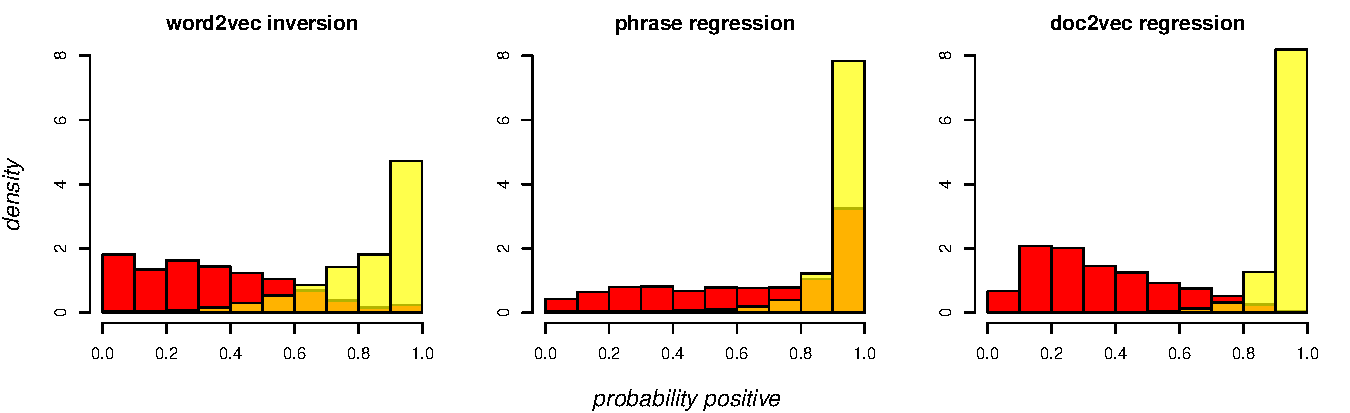
\includegraphics[width=\textwidth]{../graphs/coarseprob}

\vskip .5cm
\begin{center}
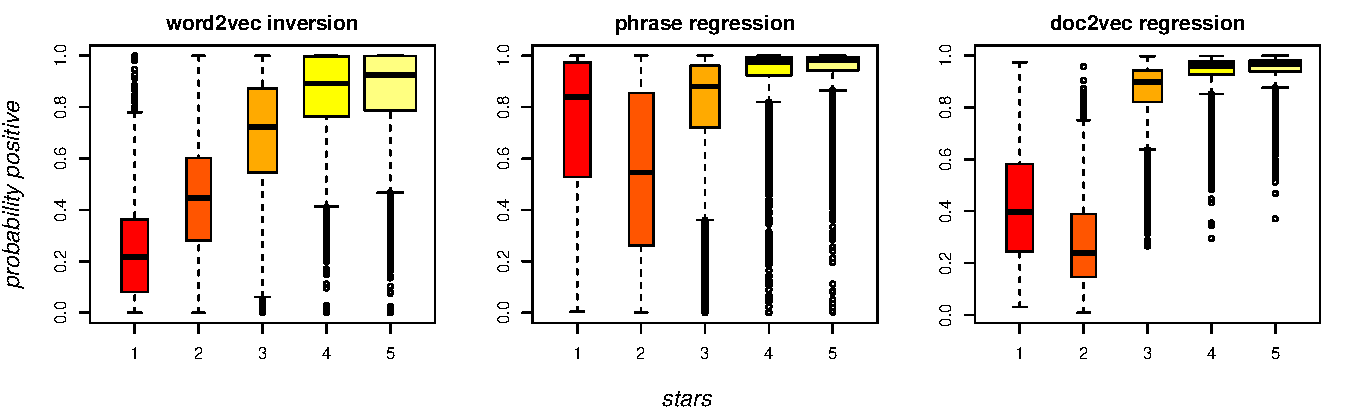
\includegraphics[width=.98\textwidth]{../graphs/coarseprob_bystar}
\end{center}
\vskip -.25cm
\caption{\label{pic:coarseprob} Out-of-Sample fitted probabilities of a review having greater than 2 stars. In the top histograms, red (dark) are the probabilities for true negative reviews and yellow (light) are for true positives.}
\end{figure*}
 


\begin{figure*}
\begin{center}
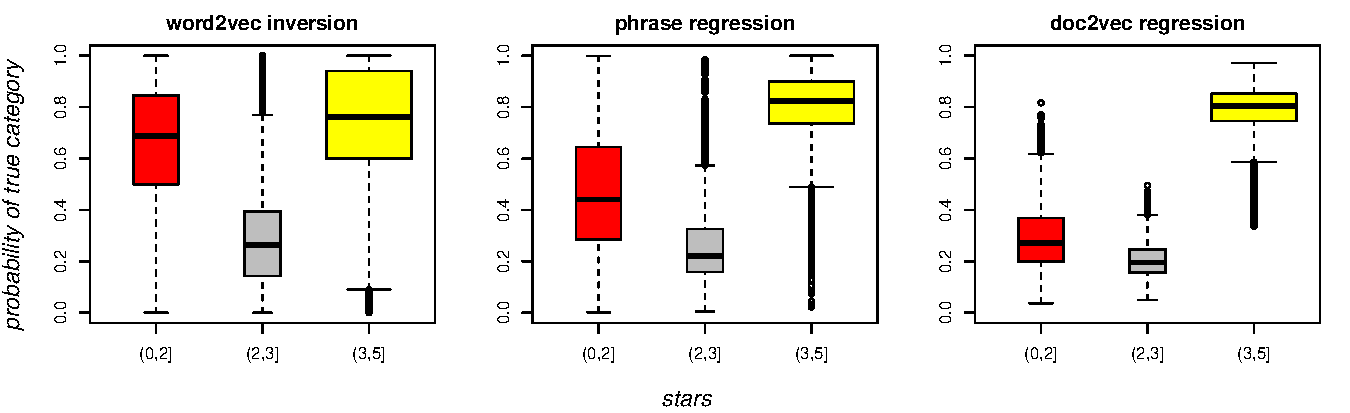
\includegraphics[width=.98\textwidth]{../graphs/nnpprob}

\vskip .25cm

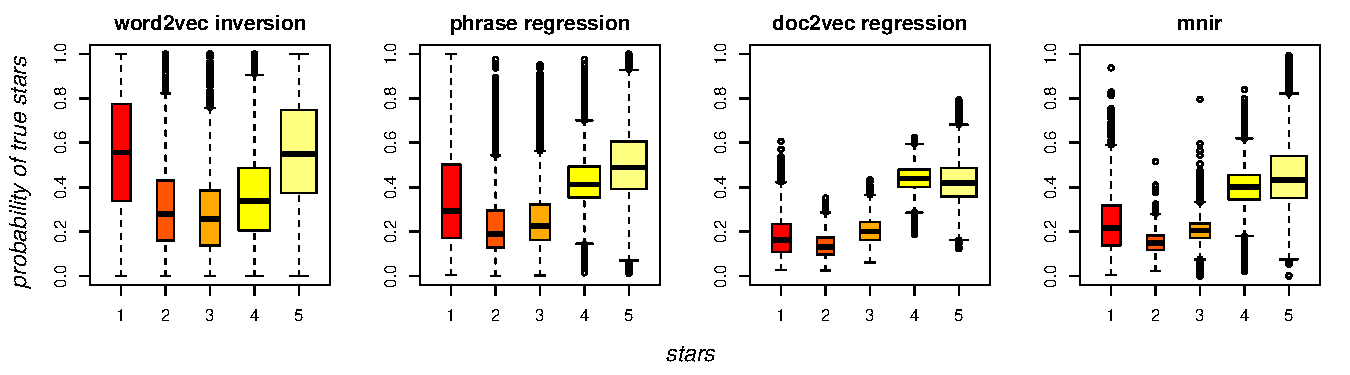
\includegraphics[width=.98\textwidth]{../graphs/fineprob}
\end{center}
\vskip -.25cm
\caption{\label{pic:fineprob} Out-of-Sample fitted probabilities for  observed truth.  In the top plot, we are predicting Negative ($\leq 2$), Neutral ($3$), or Positive ($\geq 4$).  In the bottom, we are predicting each of the separate 5 star ratings.}
\end{figure*}
 
\section{Discussion}

generative vs discrimative, quality of classification probabilities as inputs to larger systems.

\bibliographystyle{acl}
\bibliography{deepir}


\end{document}
